%!TEX root = main.tex

In this section, we introduce \textbf{A}ndroid \textbf{S}tack \textbf{M}achine (\AMASS), a formal model to capture the Android multitasking mechanism. 
%The {\AMASS} model is the same as that in \cite{HC+19} and strictly extends that in \cite{CHS+18}.  
%is inspired by the previous work~\cite{ChenHSWWY18,HCWWY19}, but the model significantly deviates from the ASM therein. 

Following the overview of Section~\ref{sec:amm}, we shall concentrate on the launch mode, the task affinity, and the intent flags when an activity is launched.  There are four launch modes in Android: ``standard (STD)'', ``singleTop (STP)'', ``singleTask (STK)'' and ``singleInstance (SIT)''.  
Furthermore, Android provides 23 intent flags related to activities,\footnote{https://developer.android.com/reference/android/content/Intent\#flags}
%\cite{intent-flags}, 
namely, the flags whose names start with $\rm FLAG\_ACTIVITY$. %among which 19 flags contain ACTIVITY in their
%names  
Among these 23 intent flags, we consider the following five that are commonly used in Android apps, namely,
\begin{itemize}
	\item $\rm FLAG\_ACTIVITY\_NEW\_TASK$ ($\ntkflag$),
	\item $\rm FLAG\_ACTIVITY\_CLEAR\_TOP$ ($\ctpflag$),
	\item $\rm  FLAG\_ACTIVITY\_SINGLE\_TOP$ ($\stpflag$),
	\item $\rm  FLAG\_ACTIVITY\_CLEAR\_TASK$ ($\ctkflag$),
	% \item $\rm FLAG\_ACTIVITY\_MULTIPLE\_TASK$ ($\mtkflag$),
	\item $\rm FLAG\_ACTIVITY\_REORDER\_TO\_FRONT$ ($\rtfflag$),
	% \item $\rm FLAG\_ACTIVITY\_TASK\_ON\_HOME$ ($\tohflag$).	
	%\item $FLAG\_ACTIVITY\_EXCLUDE\_FROM\_RECENTS$ (FAEFR),
	%	\item $\dots$.
\end{itemize}

Let $\flagset=\{\ntkflag, \ctpflag, \stpflag, \ctkflag, \rtfflag \}$ denote the set of intent flags, $\bool(\flagset)$ denote the set of formulae $\phi = \bigwedge \limits_{F \in \flagset} \theta_F$, where $\theta_F = F$ or $\neg F$. For convenience, we use $\bot$ to denote $ \bigwedge \limits_{F \in \flagset} \neg F$. 

\begin{definition}[Android Stack Machine, \AMASS] \label{def:afsm}
An {\AMASS} is a tuple $\Mm = (\act, A_0, \lmd, \aft, \Delta)$, where 
\begin{itemize}
\item $\act$ is a finite set of activities, and $A_0 \in \act$ is the main activity. Let $m=|\act|$.
\item $\lmd : \act \rightarrow \{\standard,\singletop,\singletask,\singleinstance\}$ is the launch-mode function,
%
\item $\aft : \act \rightarrow [m]$ is the task-affinity function, 
% for each activity $A$ with $\lmd(A) = \SIT$, $\aft(A)$ is unique,
%
\item $\Delta \subseteq \{\back\} \cup \act \times \{\startactivity(A,\phi)\mid A \in \act, \phi \in \bool(\flagset)\}$ is a finite set of transition rules.
%$(\beta_1(F_1, i_1), \cdots, \beta_k(F_k, i_k))$ such that for each $j \in [k]$, $\beta_j \in \{\ADD,\REM, \REP\}$, $F_j \in \frag$, and $i_j \in \Nn$. 
\end{itemize}
%
\end{definition}
We use $\act_{\star}$ to denote $\{B\in\act\mid \lmd(B)= \star\}$ for $\star\in\{\STD,\STP,\STK,\SIT\}$.
For readability, we write a transition rule $(A, \startactivity(B, \phi))\in \Delta$ as $A \xrightarrow{\startactivity(\phi)} B$


%%%%%%%%%%%%%%%%%%%%%%%%%%%%%%%%%%%%%%%%%%%
%\subsection{Semantics of \AMASS}\label{sec:semantics-amass}


%Let us first introduce some notations to be used in the definition of the semantics.

\paragraph{Tasks and configurations} A \emph{task} of $\Mm$ is encoded as a pair $(S, \aname)$, where $S= [A_1, \cdots, A_n] \in \act^+$ denotes the content of the stack, with $A_1$ (resp. $A_n$) as  the top (resp. bottom) symbol, denoted by $\topact(S)$ (resp. $\btmact(S)$), and $\aname$ is the affinity of the task, namely, the affinity of the activity which was pushed into the task when the task was created. A task $(S, \aname)$ is called an $\SIT$-task if $\lmd(\btmact(S)) = \SIT$.
%We define the \emph{affinity of a task} $S$, denoted by $\aft(S)$, to be $\aft(\btmact(S))$. 
For $S_1 \in \act^+$ and $S_2 \in \act^+$, we use $S_1 \cdot S_2$ to denote the concatenation of $S_1$ and $S_2$.

A \emph{configuration} of $\Mm$ is $\rho = ((S_1,\aname_1), \cdots, (S_n,\aname_n))$ such that
\begin{itemize}
\item for each $i \in [n]$, $(S_i,\aname_i)$ is a task, $S_i = [A_{i,1}, \cdots, A_{i, m_i}]$ is a task and $\aname_i$ is the task affinity of $S_i$ for each $i \in [n]$, moreover, 
%
\item for each $1 \le i < j \le n$ such that $(S_i, \aname_i)$ and $(S_j, \aname_j)$ are non-$\SIT$ tasks,  we have $ \aname_i \neq \aname_j$.  (Intuitively, the task affinities of every two non-$\SIT$ tasks are different. )
\end{itemize}
The task $(S_1,\aname_1)$ and $(S_n,\aname_n)$ are called the \emph{top task} and the \emph{bottom task} respectively. 
%The \emph{task affinity} of a task is the task affinity of the activity which was pushed into the task as the bottom activity when the task is created. 


% Let $\conf_{\Mm}$ denote the set of configurations of $\Mm$. 
Let $\confs(\Mm)$ denote the set of configurations of $\Mm$.
The initial configuration is $(([A_0],\aft(A_0)))$ which contains one task $([A_0], \aft(A_0))$ only. 
% Let $\confs(\Mm)$ denote the set of configurations $\rho$ such that $([A_0])\rightarrow_{\Mm}^*\rho$.

We shall define the semantics of an {\AMASS} $\Mm$ as a transition relation $\rho \xrightarrow[\Mm]{\tau} \rho'$, where $\tau \in \Delta$ is a transition rule, $\rho \in \confs(\Mm)$, and $\rho' \in \confs(\Mm)$ is obtained by applying $\tau$ to $\rho$. Moreover, it is not hard to verify that the transition relation $\xrightarrow[\Mm]{\tau}$ preserves the invariant of configurations, that is, if $\rho$ satisfies that the task affinities of every two non-$\singleinstance$ tasks are different, and $\rho \xrightarrow[\Mm]{\tau} \rho'$ for some $\tau$, then $\rho'$ satisfies this invariant as well. 

%\paragraph{Transition relation} 
We define the relation $\xrightarrow[\Mm]{}$ which comprises the quadruples $(\rho, \tau, \rho') \in \conf_\Mm \times \Delta  \times \conf_\Mm$ to formalise the semantics of $\Mm$. For readability, we write $(\rho, \tau, \rho')\in\ \xrightarrow[\Mm]{}$  as $\rho \xrightarrow[\Mm]{\tau} \rho'$. 
Let $\xRightarrow[\Mm]{}$ denote the reflexive and transitive closure of $\xrightarrow[\Mm]{}$.

\paragraph{Task allocation mechanism} 
%Via extensive experiments, we identify a crucial notion, i.e., task affinity of tasks, which plays a pivotal role in such a mechanism.
When an activity is launched, it may not be put in the top task. 
When an activity $B$ is launched and not going to be put in the top task, the following rules are used to determine which task will it be allocated. 
\begin{itemize}
	\item In case $\lmd(B) \neq \SIT$, if there is a non-$\SIT$-task whose task affinity is the same as $B$, then $B$ will be put on the task; otherwise, a new task will be created to hold $B$.
 
	\item In case $\lmd(B) = \SIT$,    if there is any task whose bottom activity is $B$ (actually $B$ is the only activity in the task), then the task will be moved to the top; otherwise, a new task is created to hold $B$.
\end{itemize}


It turns out that the semantics of {\AMASS} is highly complicated due to the complex interplay between launch modes and intent flags. Therefore, in the sequel, we separate the concerns further and consider the two sub-models of $\AMASS$, namely $\LMAMASS$ and $\IFAMASS$, which focus on launch modes and intent flags of $\AMASS$ respectively. 
More precisely, 
\begin{itemize}
	\item an $\LMAMASS$ is an $\AMASS$ $\Mm = (\act, A_0, \lmd, \aft, \Delta)$ where all the transition rules $A \xrightarrow{\alpha(\phi)} B$ (except $\back$) satisfy that $\phi = \bot$, 
	\item an $\IFAMASS$ is an $\AMASS$ $\Mm = (\act, A_0, \lmd, \aft, \Delta)$ where all the activities $A\in\act$ satisfy that $\lmd(A) = \STD$ and $\aft(A) = \aft(A_0)$.
\end{itemize}
To ease the understanding, in the sequel, we shall define the semantics of the two sub-models $\LMAMASS$ and $\IFAMASS$ first, then define the semantics of $\AMASS$. 



	
%%%%%%%%%%%%%%%%%%%%%%%%%%%%%%%%%%%%%%%%%%%%%%%%%%%%%%%%%%%%%%%%%%%%%%%%%%%%%%%%%%%%%%

%%%%%%%%%%%%%%%%%%%%%%%%%%%%%%%%%%%%%%%%%%%%%%%%%%%%%%%%%%%%%%%%%%%%%%%%%%%%%%%%%%%%%%

%As we have seen, 
The semantics of {\AMASS} %in Section~\ref{sec:amass} 
is rather complicated and it is highly challenging to achieve a decision procedure for the configuration reachability problem of {\AMASS}. 
%
In this paper, we restrict our attention to a sub-model of {\AMASS}, called $\STK$-dominating {\AMASS}, and design a decision procedure for it. 
%We shall see later on that the decision procedure for the sub-model is already quite involved and requires nontrivial novel ideas.  
	
	%Due to the semantics of {\AMASS} defined in Section~\ref{sec:semantics-amass} is highly complicated, it is difficult to provide a decision algorithm for solving the configuration reachability problem of {\AMASS}. To this end, we introduce a fragment of {\AMASS} called STK-dominating {\AMASS}, which accommodates all launch mdoes and intent flags. 
	
	\begin{definition}[$\STK$-dominating \AMASS] \label{def:stk-amass}
		Let $\Mm = (\act, A_0, \lmd, \aft, \Delta)$ be an $\AMASS$. Then $\Mm$ is  said to be \emph{$\STK$-dominating} if the following constraints are satisfied.
		\begin{enumerate}
			\item $\back\in\Delta$,
			\item the task affinities of $\singletask$-activities (if there is any) are mutually distinct,
			%        \item for each transition $A \xrightarrow{\startactivity(\phi)} B\in\Delta$ such that $A\in\act_{\singleinstance}$, it holds that $B\in\act_{\singleinstance}\cup\act_{\singletask}$,
			\item for each transition $A \xrightarrow{\startactivity(\phi)} B\in\Delta$ such that $A \in \act_\singleinstance$ or $\phi\models \ntkflag$, we have $B \in \act_{\singleinstance} \cup \act_{\singletask}$.
		\end{enumerate}
	\end{definition}
	Intuitively, in an $\STK$-dominating $\AMASS$ $\Mm$, the task creation or task switching actions are all triggered by the $\singleinstance$ or $\singletask$ launch mode, more precisely,  
	each task of $\Mm$ contains at most one $\STK$-activity, moreover, whenever a task creation or task switching action occurs, the launched activity is of $\singleinstance$ or $\singletask$ launch mode, equivalently speaking, 
	whenever an $\standard$ or $\singletop$-activity is started, no task creation or task switching actions occur.  %This intuition is formalized by the proposition below.
	%For the two sub-models of $\AMASS$, i.e., $\LMAMASS$ and $\IFAMASS$, an $\LMAMASS$ (resp. $\IFAMASS$) is said to be $\STK$-dominating if the above four constraints are satisfied.
	
	\begin{example}
		We will use the following example to illustrate the concept of $\STK$-dominating $\AMASS$.
		Let $\Mm=(\act,A,\lmd,\aft,\Delta)$, where 
		\begin{itemize}
			\item $\act = \{A, B, C, D, E\}$, 
			%
			\item $\lmd(A)=\lmd(B)=\standard$, $\lmd(C) = \singleinstance$, $\lmd(D) = \lmd(E) = \singletask$, 
			%
			\item $\aft(A) = 0$, $\aft(B) = \aft(C) = 1$, $\aft(D) = 2$, $\aft(E) = 3$, 
			%
			\item $\Delta = \{\back,\tau_1, \tau_2, \tau_3, \tau_4, \tau_5, \tau_6\}$, where 
			\begin{itemize}
				\item 	$\tau_1 = A \xrightarrow{\startactivity(\ntkflag)} C$,
				$\tau_2 = B \xrightarrow{\startactivity(\ntkflag)} E$,
				$\tau_3 = C \xrightarrow{\startactivity(\bot)} D$,
				\item		$\tau_4 = C \xrightarrow{\startactivity(\bot)} C$,
				$\tau_5 = D \xrightarrow{\startactivity(\ctpflag)} B$,
				$\tau_6 = E \xrightarrow{\startactivity(\bot)} D$. 
			\end{itemize}
		\end{itemize}
		Then $\Mm$ is an $\STK$-dominating {\AMASS}, since
		\begin{itemize}
			\item in $\tau_1 = A \xrightarrow{\startactivity(\ntkflag)} C$, $\lmd(C) = \singleinstance$,  
			%
			\item in $\tau_2 = B \xrightarrow{\startactivity(\ntkflag)} E$, $\lmd(E) = \singletask$, 
			%
			\item in $\tau_3 = C \xrightarrow{\startactivity(\bot)} D$, $\lmd(C) = \singleinstance$ and $\lmd(D) = \singletask$, 
			%
			\item in $\tau_4 = C \xrightarrow{\startactivity(\bot)} C$, $\lmd(C) = \singleinstance$. 
		\end{itemize}
		The configurations that are reachable from the initial configuration $(([A_0], 0))$ are illustrated in Figure~\ref{stk-asm-example}, where the vertices denote the configurations and the edges denote the elements of $\xrightarrow[\Mm]{}$. 
		Note that for $\Mm$, there are only finitely many configurations reachable from the initial configuration.  
		\begin{figure}[htbp]
			% \vspace{-3mm}
			\centering
			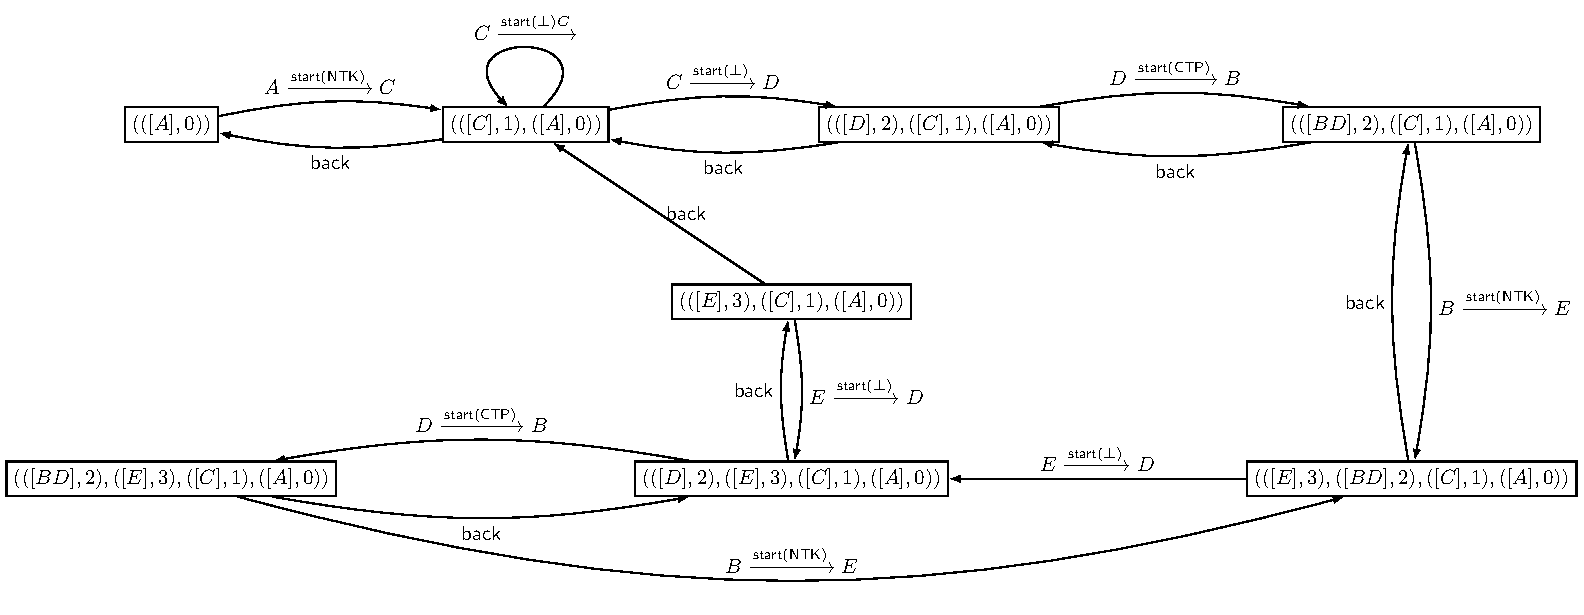
\includegraphics[scale = 0.5]{stk-asm-example.pdf}
			\caption{Configurations that are reachable from the initial configuration $(([A_0], 0))$ in the $\STK$-dominating $\AMASS$ $\Mm$}
			%in $\phi$
			% \vspace{-6mm}	
			\label{stk-asm-example}
		\end{figure}
		
		%\begin{table}[htbp]
		%	\begin{center}
			%	\begin{tabular}{|c|c|c|c|c|c|}
				%	\hline
				%	Activity & $\lmd$ & $\aft$\\
				%	\hline
				%	$A$ & $\STD$ & 0\\
				%	\hline
				%	$B$ & $\STP$ & 1 \\
				%	\hline
				%	$C$ & $\SIT$ & 1 \\
				%	\hline
				%	$D$ & $\STK$ & 2 \\
				%	\hline
				%	$E$ & $\STK$ & 3 \\
				%	\hline
				%	\end{tabular}
			%	\caption{Attributes of activities}
			%	\label{tab-attribute-stk}
			%	\end{center}
		%\end{table} 
	\end{example}


%%%%%%%%%%%%%%%%%%%%%%%%%%%%%%%%%%%%%%%%%%%%%%%%%%%%%%%%%%%%%%%%%%%%%%%%%%%%%%%%%%%%%%


\smallskip
\noindent\textbf{Configuration reachability problem of $\AMASS$} %\label{sec-conf-reach}

In this paper, we focus on the configuration reachability problem of $\AMASS$. This problem is fundamental to the formal (static) analysis and verification of the behaviors of Android apps with respect to the multitasking mechanism.  

Let $\Mm =(\act, A_0, \lmd, \aft, \Delta)$ be an  {\AMASS}. Then we define $\RConfs(\Mm)$ as the set of configurations $\rho$ that are reachable from the initial configuration, that is, 
$(A_0, \aft(A_0)) \xRightarrow[\Mm]{} \rho$. 
Let $(\Aut_1,\cdots,\Aut_k)$ be an {\NFA} tuple over the alphabet $\act$. We define $\Rel((\Aut_1, \cdots, \Aut_k))$ as $(S_1, \cdots, S_k)$ such that for each $i \in [k]$, $S_i \in \Lang(\Aut_i)$. Moreover, let $\theta = \aname_1\cdots\aname_k$ be an affinity sequence. Then $\confs((\theta, (\Aut_1,\cdots,\Aut_k)))$, \emph{the set of configurations accepted by $(\theta, (\Aut_1,\cdots,\Aut_k))$}, is defined as as the set of configurations $\rho = ((S_1,\aname'_1),\cdots,(S_k,\aname'_k))$  such that $(S_1, \cdots, S_k) \in \Rel((\Aut_1, \cdots, \Aut_k))$, and for each $i \in [k]$, $\aname_i=\aname_i'$.
%
% $\confs((\theta, (\Aut_1,\cdots,\Aut_k)))$, \emph{the set of configurations accepted by $(\theta, (\Aut_1,\cdots,\Aut_k))$}, as the set of configurations $\rho = ((S_1,\aname'_1),\cdots,(S_k,\aname'_k))$  such that for each $i \in [k]$, $\aname_i=\aname_i'$ and $S_i \in \Lang(\Aut_i)$. 
Then \emph{the configuration reachability problem} of {\AMASS} is defined as follows. 
\begin{quote}
	Given an {\AMASS} $\Mm= (\act, A_0, \lmd, \aft, \Delta)$, an affinity sequence $\theta = \aname_1\cdots\aname_k$, and an {\NFA} tuple $(\Aut_1,\cdots,\Aut_k)$ over the alphabet $\act$, decide whether $ \confs({(\theta, (\Aut_1,\cdots,\Aut_k))}) \cap \RConfs(\Mm) \neq \emptyset$.
\end{quote}


%%%%%%%%%%%%%%%%%%%%%%%%%%%%%%%%%%%%%%%%%%%%%%%%%%%%%%%%%%%%%%%%%%%%%%%%%%%%%%%%%%%%%%

